\documentclass[10pt,twocolumn,letterpaper]{article}

\usepackage{cvpr}
\usepackage{times}
\usepackage{epsfig}
\usepackage{graphicx} %package to manage images
\graphicspath{{images/}}
\usepackage[english]{babel}
\usepackage[autostyle, english = american]{csquotes}
\MakeOuterQuote{"}
\usepackage{amsmath}
\usepackage{amssymb}
\usepackage{caption}
\captionsetup[table]{skip=5pt}

\usepackage{float}

% Include other packages here, before hyperref.

% If you comment hyperref and then uncomment it, you should delete
% egpaper.aux before re-running latex.  (Or just hit 'q' on the first latex
% run, let it finish, and you should be clear).
\usepackage[breaklinks=true,bookmarks=false]{hyperref}

\cvprfinalcopy{} % *** Uncomment this line for the final submission

\def\cvprPaperID{****} % *** Enter the CVPR Paper ID here
\def\httilde{\mbox{\tt\raisebox{-.5ex}{\symbol{126}}}}

% Pages are numbered in submission mode, and unnumbered in camera-ready
%\ifcvprfinal\pagestyle{empty}\fi
\setcounter{page}{1}
\begin{document}

%%%%%%%%% TITLE
\title{A comparison of classification techniques for determining the proximity
of restaurants to college campuses based on their Yelp information}

\author{Daniel Wen, Jimmy Zhu, Kwesi Rutledge\\
  University of California, San Diego\\
  {\tt\small \{dhwen,jmz005,krutledg\}@eng.ucsd.edu}
  % For a paper whose authors are all at the same institution,
  % omit the following lines up until the closing ``}''.
  % Additional authors and addresses can be added with ``\and'',
  % just like the second author.
  % To save space, use either the email address or home page, not both
  %\and
  %Jimmy Zhu\\
  %UC San Diego\\
  %{\tt\small jmz005@eng.ucsd.edu}
  %\and
  %Kwesi Rutledge\\
  %UC San Diego\\
  %{\tt \small krutledg@eng.ucsd.edu}
}

\maketitle
%\thispagestyle{empty}

%%%%%%%%% ABSTRACT
\begin{abstract}
  We attempt to investigate whether a restaurant can be identified to be within
  a close proximity of a college campus based on their Yelp review data. We
  employ a discriminant distance threshold of around 5 miles, chosen by
  cross-validation, and assign labels for college- and non-college-oriented
  businesses based on this delimiter. We will use an ensemble of popular
  classification techniques on a feature set representing check-in periods and
  review text and separately compare their performances in classification.
\end{abstract}

%%%%%%%%% BODY TEXT
\section{Introduction}

Dining cultures around the world are largely shaped by the demographics that
they serve. Based on varying incomes, cultural composition, and work-life
schedules, restaurants, like all businesses, need to tailor their experiences
with the customer in mind. Our principle investigation entails a study on
whether distinctions can be identified between restaurants that cater towards a
college based population compared to restaurants elsewhere. To assist us in our
effort, we will use a comprehensive dataset from Yelp containing restaurant
information on over 8000 establishments around the country along with a
collection of popular generative and discriminant classification techniques to
see if we can determine a methodology for labeling a restaurant as
college-oriented or not college-oriented.


\section{Description}

We work with an extensive data collection provided by Yelp as part of their
official 2016 Dataset Challenge. This database contains a wealth of information
on over 9000 restaurants located throughout several major US cities; it contains
extensive information per establishment detailing  customer check-in hours,
transcripts of user reviews, review ratings, business tags, and geographical
locations.

The coordinates of the Universities were retrieved through consultation with the Institute of Education Sciences, a government based group with ownership of a comprehensive database of the longitudinal and latitudinal positions on every academic institution in the country (which includes specialty schools and technical institutes). We parsed through the complete listing of their academic collection and extracted the geographical positions on just the traditional 4-year universities.

With the location data on the college campuses available, we are able to calculate
the distance between a restaurant and any nearest university. For
labelling a restaurant within the college and non-college based classes, we
choose a tentative threshold distance that will be evaluated statistically on a
maximum likelihood basis. Our intent and choices for the features to be
classified along with approaches for representation are detailed in the
following subsections.

\subsection{Check-in Hours}

The check-in data from the Yelp database came as a collection of histograms
detailing the frequency of check-ins over incremental hour slots throughout the
week. A direct representation of the histogram data made for a very sparse list,
with most of the hour slots being empty. To resolve this, we grouped the
check-in counts for multiple hours into larger time slots to reduce both the
size and the sparsity of the feature vector.

In order to normalize this feature set, we applied Fisher's linear discriminant to modify the check-in data into a single dimensional direction which maximizes discriminants between our classes.

\subsection{Restaurant Tags}

The choice of representation of Restaurant Tags is unique in the sense that they are not numerical. There is a fairly large number of these categories within our Yelp Data; to account for each unique category and to avoid the notions of "closeness" or
"proximity" that come with assigning each tag a number (e.g. from 1 to C, where C is
the number of categories), we chose an orthogonal representation of all the
restaurant tags.

This means assigning each category an index in each business vector
(i.e.\ entry 257 will always be the entry for the "Indian Food" tag in every
business) and placing a 1 or 0 in that entry for a restaurant depending on whether or not the tag was present or not.

\subsection{Review Context}

To parse the contextual information within the reviews, we leveraged the latent
Dirichlet allocation algorithm designed by Blei~et.\ al~\cite{LDA_original} to
categorize the written text into subtopics. We modeled the collective reviews of
a business as a corpus and the individual reviews as documents in the corpus. We
set a topic count of 3 topics per business and identified the top 8 words
associated with the LDA discovered topics.\\

\begin{table}[H]
  \centering
  \begin{tabular}{|r|l|}
    \hline
    Topic 1 & donut, dunkin, locat, t, get, one, custom\tabularnewline
    \hline
    Topic 2 & s, morn, nice, place, coolata, stop, new \tabularnewline
    \hline
    Topic 3 & coffe, servic, good, time, go, food, back\tabularnewline
    \hline
  \end{tabular}
  \caption{Subtopic generation via LDA}\label{table:LDA_example}
\end{table}


The above table shows an example of the output of subtopic extraction performed
on a suburban cafe. Notice how some of the words are grammatically incoherent;
this is because both stemming and stop-word filtering was applied on the data
set which rooted redundant phrases and removed uninformative function words
(e.g.\ is, which, that). Intuitively, we can still infer some themes according to
the identifiable words which arguably represent topics of "Food Selection",
"Ambience", and "Experience" for topics 1 through 3 respectively.

With the subtopic words extracted from the training set, we create a dictionary
of terms for mapping. This is a grow-able list which can be appended from
information provided in future training data, but for the time being it is
composed of purely the vocabulary selection from the available terms. Each
subtopic grouping for a particular business in the training and test sets is
represented by a vector with dimensionality equal to the vocabulary size and a
value of 1 at each index where a term is present and 0 otherwise. This quantized
subtopic vector is finally treated with FLD to reduce overall dimensionality.

\section{Experimental Results}

The problem can be seen as a typical classification problem in which we wish to
determine labels of "college-oriented" or "not college-oriented" using a
restaurant's Yelp data.

Since the raw Yelp data does not already include these labels, this appears to
be an unsupervised learning problem. However, to simplify the problem, we decided
to add these missing labels ("college" vs.\ "not college") to the Yelp data set,
basing them solely on the distance of each restaurant to the nearest college
campus. Data points are assigned to either the "college" class if the
restaurant lies within a chosen distance threshold, or to the "not-college"
class if the restaurant exceeds that threshold.

Since there are many potential choices to use for the distance threshold, we
opted to select this parameter experimentally. Using a simple Gaussian
classifier, we varied the distance threshold used to separate the training data,
which resulted in different error rates for each threshold chosen. Based on
these error rates, we were able to qualitatively select an optimal threshold of
5.2 miles.

After separating the training and test data based on this optimal threshold, we
then applied more sophisticated classification techniques to the problem,
including both AdaBoost and neural networks.

\subsection{Gaussian BDR and Threshold Selection}

Out of all the classification strategies used, the simplest one to understand
and implement is the Gaussian BDR classifier. This makes it a good candidate for
cross-validating the distance threshold used to separate the two classes.

For thresholds between 1 and 10 miles, we tested the Gaussian classifier on
various representations of the training set.
Figures~\ref{fld_bdr_error_v_threshold_no_subtopics}~and~\ref{fld_bdr_error_v_threshold_yes_subtopics}
show the resulting error rate over these distance thresholds. The green and
purple curves show the estimated prior probabilities of each class as the
distance threshold changes. In each figure, a different set of features were
included in the training set.

The prior probabilities of each class $i$ are estimated by
\[
  \hat{p}_{i}=\frac{\left|\left\{ i|\mathbf{x}\in\mathcal{D}_{i}\right\} \right|}{n}\qquad n=\left|\left\{ i|\mathbf{x}\in\mathcal{D}_{0}\cup\mathcal{D}_{1}\right\} \right|
\]
where $\mathcal{D}_{i}$ is the training dataset belonging to class $i$. These
priors give an idea of what the error rate would be in the trivial case where we
simply set the decision rule to always choose class 0 or always choose 1. As
such, the green curve can be thought of as the error incurred when all samples
are classified as "not college-oriented" ($i=0$), while the purple curve shows
the error incurred when classifying all samples as "college-oriented" ($i=1$).

Looking back at the training and test set errors in
Figure~\ref{fld_bdr_error_v_threshold_no_subtopics}, we observe that the error
rate can be reduced by setting the distance threshold arbitrarily low or
arbitrarily high. However, this strategy is of no use because it suggests giving
the same classification to all training samples. This can be seen by the fact
that both the test and training error rates tend to converge on the prior
probabilities when the threshold separating the classes is too low or too high.
We can then infer that the best threshold to choose is somewhere in the middle
around 5 miles, where the BDR classification error underbounds the prior
probability curves. Based on this, we qualitatively selected a distance
threshold of 5.2 miles to separate the two classes.

\begin{figure}[h]
  \centering{}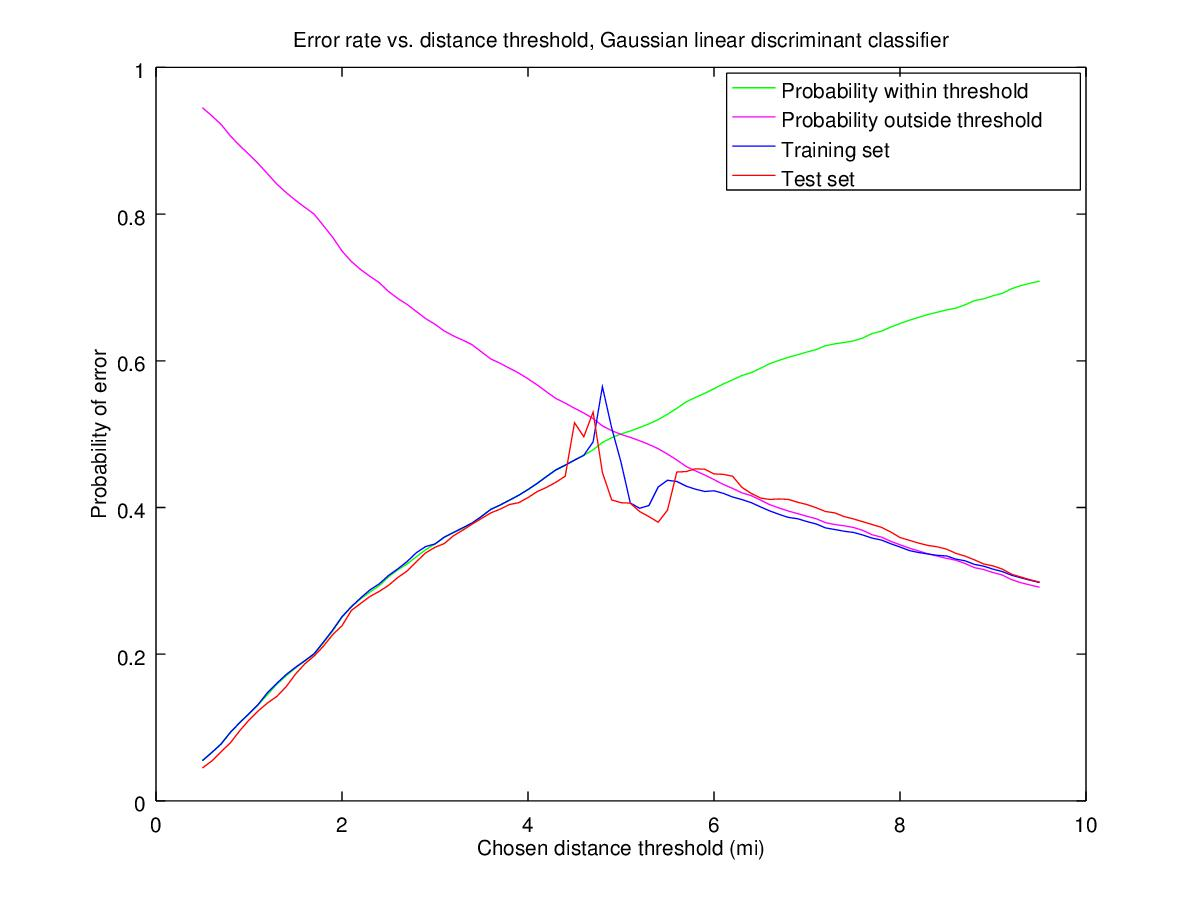
\includegraphics[width=1\linewidth]{filtered_colleges_no_subtopics/fisher_LDA_error_v_threshold}
  \caption{Features considered: check-in hours and restaurant tags.}
\label{fld_bdr_error_v_threshold_no_subtopics}
\end{figure}
\begin{figure}[h]
  \centering{}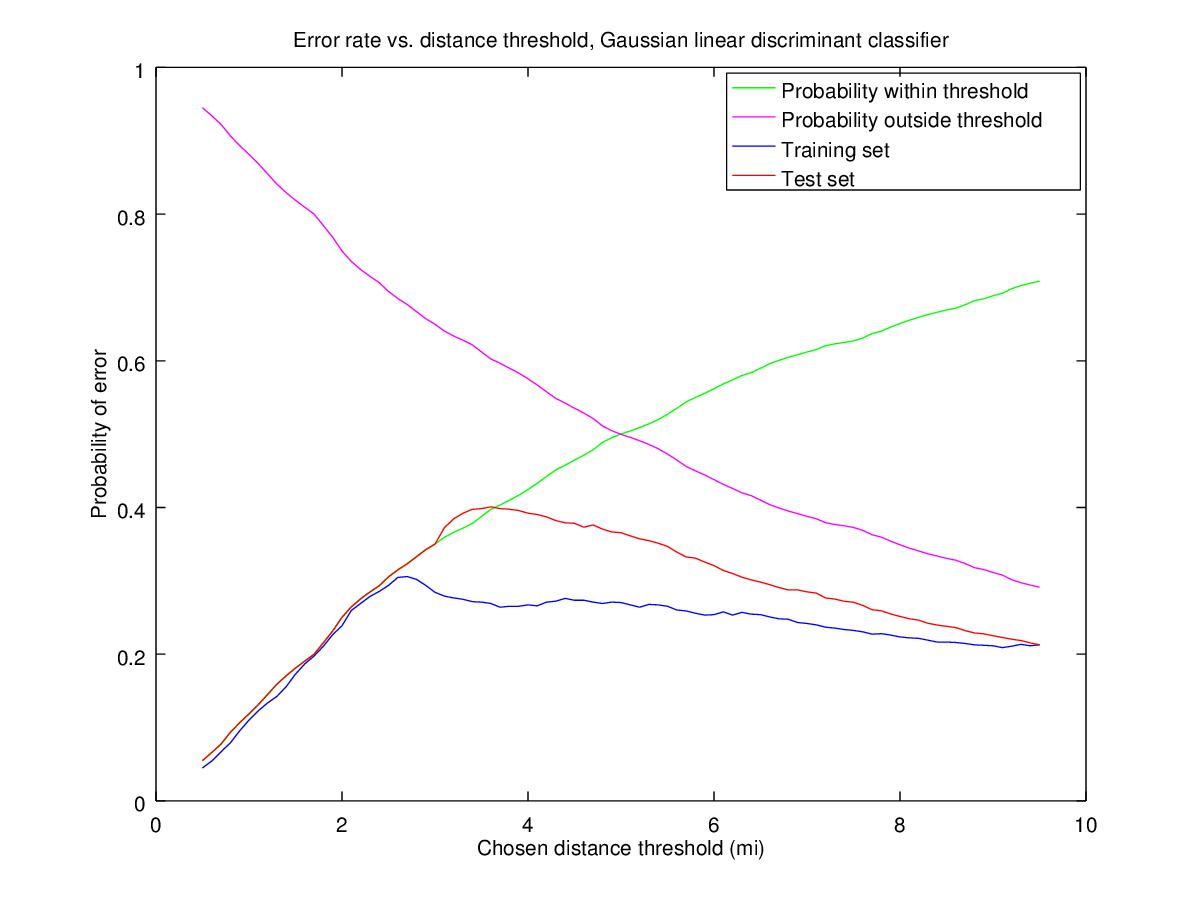
\includegraphics[width=1\linewidth]{filtered_colleges_yes_subtopics/fisher_LDA_error_v_threshold}
  \caption{Features considered: check-in hours, restaurant tags, FLD-reduced
  subtopics.}
\label{fld_bdr_error_v_threshold_yes_subtopics}
\end{figure}

In addition to finding the proper threshold, we used the Gaussian classifier to
test whether including the subtopics feature made a difference in the classifier
performance (hence the two figures for error rate vs.\ threshold). The strategy
was to classify two datasets: one without the review subtopics and one with the
subtopics.

Comparing the error rate in Figure~\ref{fld_bdr_error_v_threshold_no_subtopics}
with that of Figure~\ref{fld_bdr_error_v_threshold_yes_subtopics}, we see a
significant decrease in error when the review subtopics are included, which
validates our initial assumption that the reviews would provide valuable
information for characterizing the restaurants. This decrease in error affects a
wide range of distance thresholds, although the range 4-6 miles still appears to
be ideal. Thus, 5.2 miles seems to be a reasonable threshold in either case.

\subsection{Fisher's Linear Discriminant Analysis}

In forming the dataset of vectorized features, it was necessary to use Fisher's
Linear Discriminant (FLD) to reduce the dimensionality of the review subtopics
\cite{FLD_kernels}, since the initial representation of the subtopics resulted
in a sparse 6000-dimensional feature vector that proved to be too inefficient
for classification purposes.

Although the check-ins feature and the restaurant tags feature occupy much fewer
dimensions, it is still useful to perform FLD analysis on these features to
identify trends between college-oriented and non-college-oriented restaurants.
Since the computed FLD vector identifies discriminant features, we can look at
different segments of the discriminant vector to identify discriminant check-in
hours, discriminant restaurant tags, as well as discriminant review subtopics
that highlight the key differences between the two classes of restaurants.

For example, in Figure~\ref{checkins_discriminant}, we can observe the mean
frequency of check-ins for restaurants within the 5.2 mile college radius, as
well as the mean check-ins for restaurants outside that radius. In both classes
the peak check-in hours are concentrated around Friday and Saturday, and midday
throughout the week.

\begin{figure}[h]
  \centering{}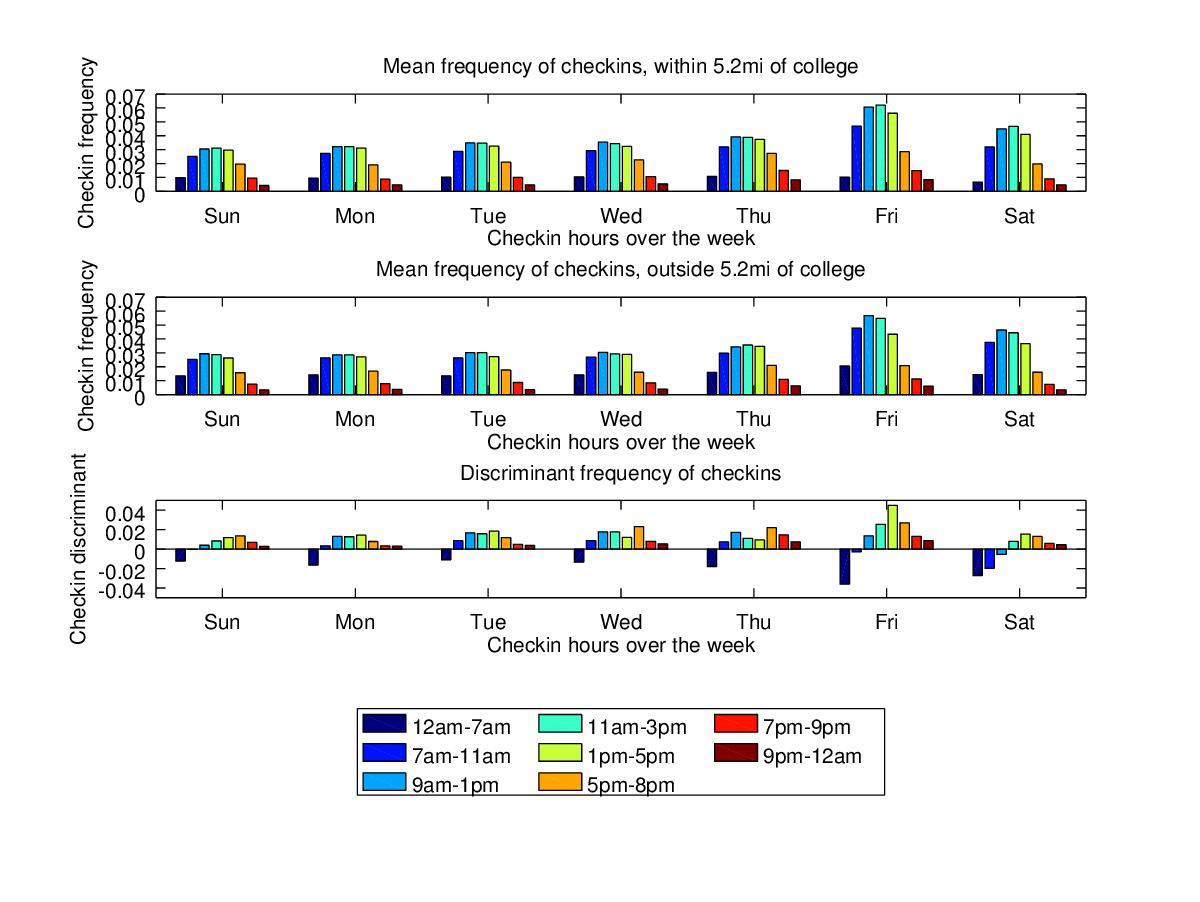
\includegraphics[width=1\linewidth]{filtered_colleges_yes_subtopics/checkins_discriminant}
  \caption{Check-in frequency of the two classes, separated by a distance
    threshold of 5.2 mi. The discriminant vector is shown in the bottom plot.}
\label{checkins_discriminant}
\end{figure}

We can also see that between 12am and 7am, restaurants near colleges receive
considerably fewer check-ins, as indicated by repeated negative discriminant
values corresponding to that time frame throughout the week, with the effect
being most pronounced on Friday. This hints at the behavior of the restaurant
clientele (college students), who appear to be significantly more active midday
on Friday than the rest of the community.

In Figure~\ref{categories_discriminant}, we notice different tags that are
commonly applied to the restaurants in both classes. Based on the discriminant
vector, the tags "Food Trucks," "Grocery," "Beer, Wine \& Spirits," and "Gas \&
Service Stations" are more common among college-oriented businesses, whereas the
tags "Coffee \& Tea," "Bakeries," "Cafes," and "Specialty Food" are more commonly
found in restaurants located outside the 5.2 mi threshold. This gives a rough
picture of the types of restaurants that tend to cluster around college
campuses (although the negative trend in "Coffee \& Tea" businesses is somewhat
surprising).

\begin{figure}[h]
  \centering{}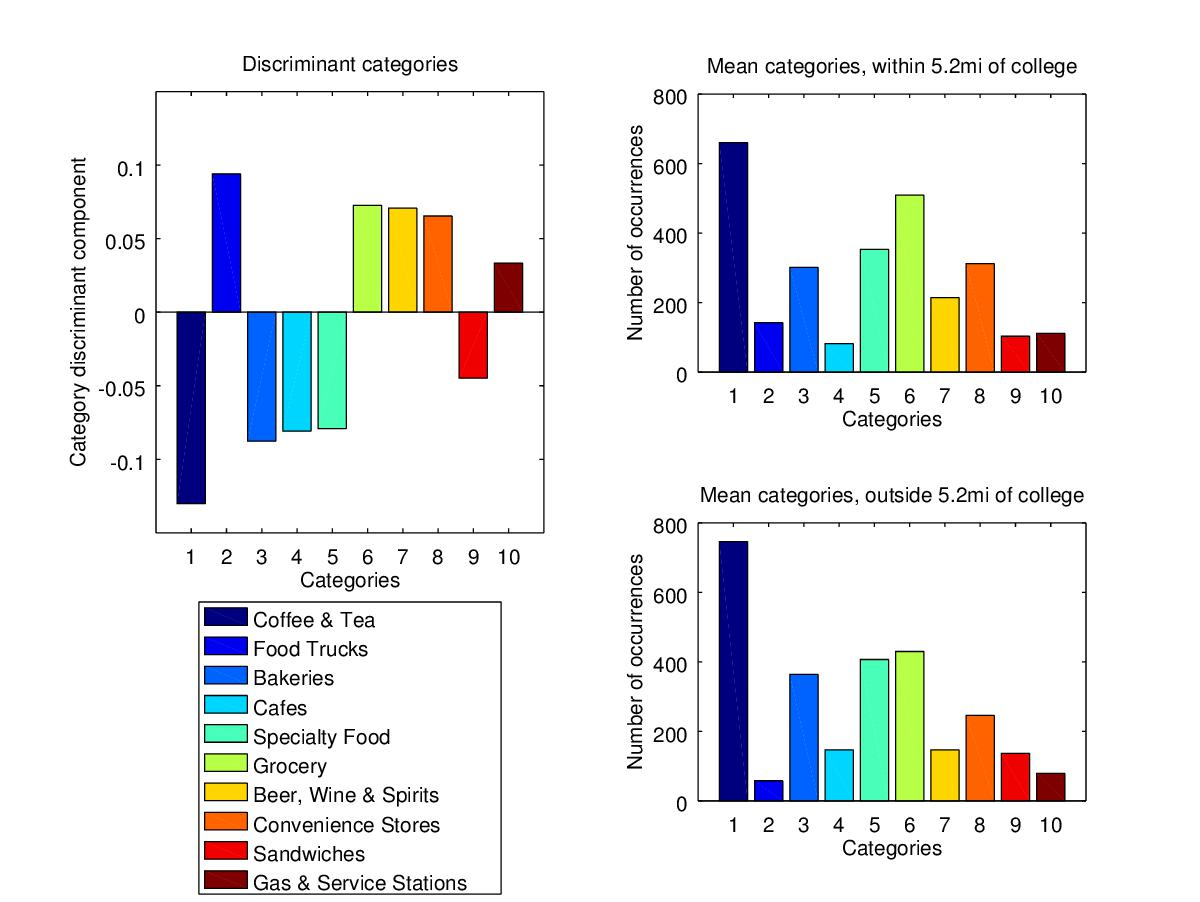
\includegraphics[width=1\linewidth]{filtered_colleges_yes_subtopics/categories_discriminant}
  \caption{Restaurant categories (tags) associated with each class, separated
    by a distance threshold of 5.2 mi. The discriminant vector shown on the left
    reveals which categories tend to belong to which class.}
\label{categories_discriminant}
\end{figure}

Finally, Figure~\ref{subtopics_discriminant} shows the review subtopics
mentioned for college-oriented and non-college-oriented businesses. In this
case, some decoding is required to understand the list of discriminant
subtopics. The topic "db" refers to "Dutch Bros Coffee," a business that appears
to be consistently outside the 5.2mi college radius, which could explain the
negative trend in the "Coffee \& Tea" tag seen in the previous figure.

The range of discriminant subtopics is extremely varied in the types of words
found. Only two discriminant subtopics are even related to food: "cinnabon" and
"greas[e]" (both with a positive trend toward college-oriented businesses).
Others are common colloquialisms and phrases "gee[z]," "luckil[y]".  And the
rest appear to be random phrases: "lb" (pounds), "happen," "garrett," etc.

The randomness of these top phrases does not give much insight into what
reviewers are actually saying about these businesses, so it is interesting that
the classifier finds these subtopics to be important, especially since the
Gaussian BDR error rate decreases significantly with the inclusion of these
subtopics. Further tweaks may be need to be made to the parameters of the latent
Dirichlet algorithm and to our vectorization of the subtopics in order to
produce more satisfactory results.

\begin{figure}[h]
  \centering{}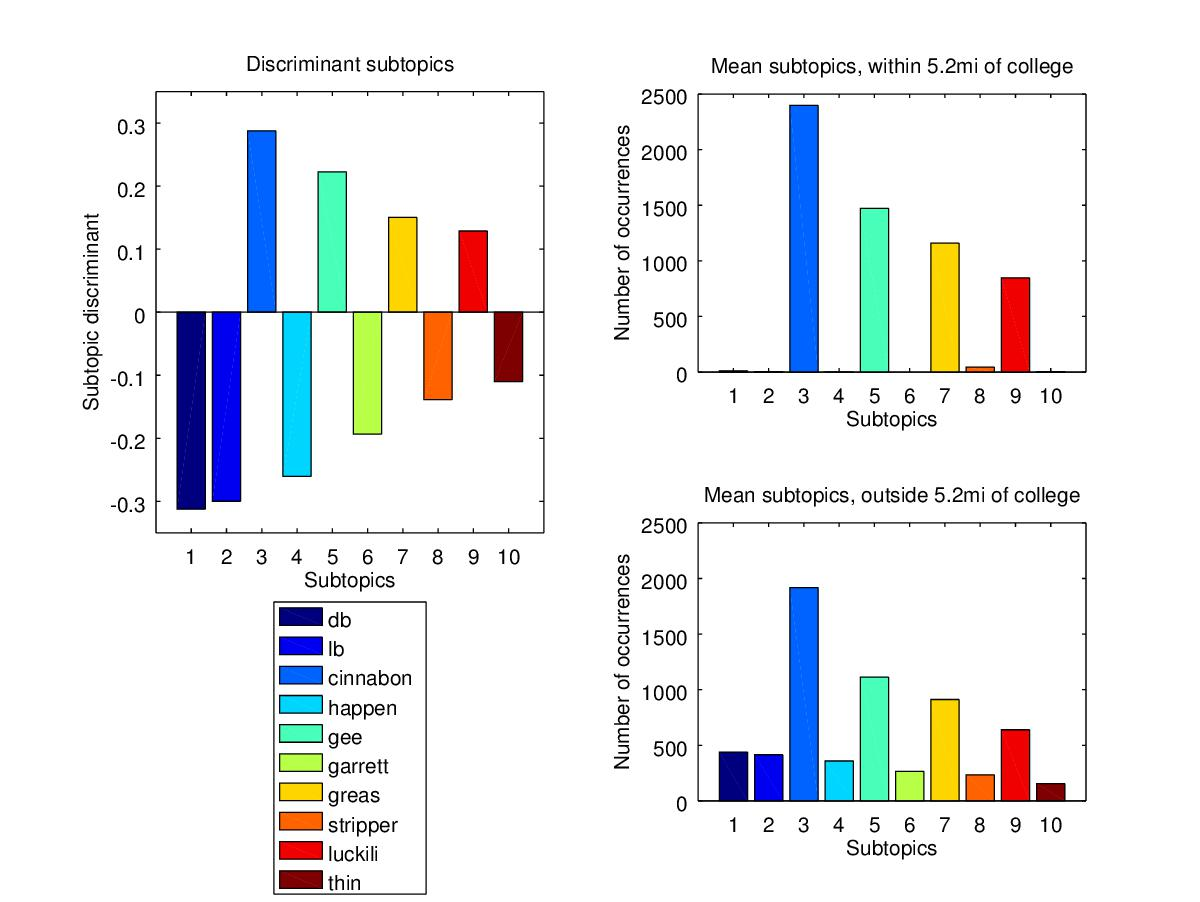
\includegraphics[width=1\linewidth]{filtered_colleges_yes_subtopics/subtopics_discriminant}
  \caption{Review subtopics associated with each class, separated by a distance
    threshold of 5.2 mi. The discriminant vector shown on the left reveals
  which subtopics tend to belong to which class.}
\label{subtopics_discriminant}
\end{figure}

\subsection{AdaBoost}

We used a slightly modified version of the AdaBoost algorithm
\cite{Adaboost_original}, in addition to do classification experiments.

This modified form included the classic exponential cost function:

$$ L[y,g(x)] = \exp( -yg(x) ) = \exp( - \gamma(x) ) $$

as well as decision stumps as the class of classifiers that we used.

\[
  \textrm{Decision Functions }
\]
\[
  u \in U = \left( u_j |
  \begin{array}{clc}
    u_j(x) & = 1,  & x_j \geq T \\
    u_j(x) & = -1, & x_j < T
  \end{array}
\right)
\]

The values of T that were chosen varied depending on the multiple versions of
our dataset that we used but I will briefly show 3 ranges that we chose. We
evenly divided each range by a set number to hopefully achieve finer distinction
between

\begin{table}[ht]
  \centering{}
  \begin{tabular}{|c|c|c|}
    \hline
    Choice & Range          & Number of Divisions\tabularnewline
    \hline
    \hline
    1      & $\{ 0, 0.02 \} $ & 50\tabularnewline
    \hline
    2      & $\{ 0, 1 \} $    & 100\tabularnewline
    \hline
    3      & $\{ -1, 1 \} $  & 200\tabularnewline
    \hline
  \end{tabular}
  \caption{Three choices for the T ranges used in our AdaBoost classifiers.}\label{table:ada_t_ranges}
\end{table}

AdaBoost, used with decision stumps within the range $ \{ 0, 1 \} $ created the
best classifier for the filtered and condensed college data, while the range of
$ \{ 0 , 0.02 \} $ created the best classifier for the unfiltered data of
check-ins paired with restaurant type. The final test error rate in both of
these cases was 36.9 and 38.38 $ \% $, respectively, at the threshold of
interest (5.2 miles).

We believe that there is still room for improvement to be made however, because
our choice of threshold ranges appeared to be overfitting in several instances.

For example, in figure~\ref{fig:adaboost_250i_example} the probability of
classification error continuously decreased over the course of our development
of the final classifier, but not while improving our performance on the test
set. Other ranges created better alignment between test error and training error
curves, so some form of cross validation or rigorous planning should be done in
the future to prevent too much overfitting.

\begin{figure}
  \centering
  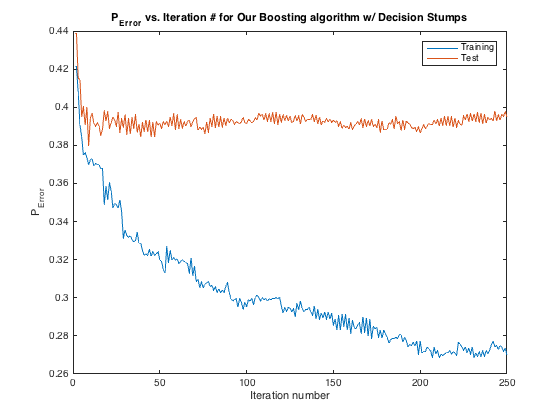
\includegraphics[width=0.9\linewidth]{adaboost_decision_stumps_0_1_250iter_filtered2}
  \caption{The AdaBoost algorithm, with many of our chosen threshold ranges, appeared to overfit our training dataset while not improving test error very much.}
\label{fig:adaboost_250i_example}
\end{figure}

The performance of the AdaBoost Algorithm over various thresholds (applied for
150 iterations at each threshold) is summarized by
Figure~\ref{fig:Adaboost_Sweep}.

\begin{figure}[H]
  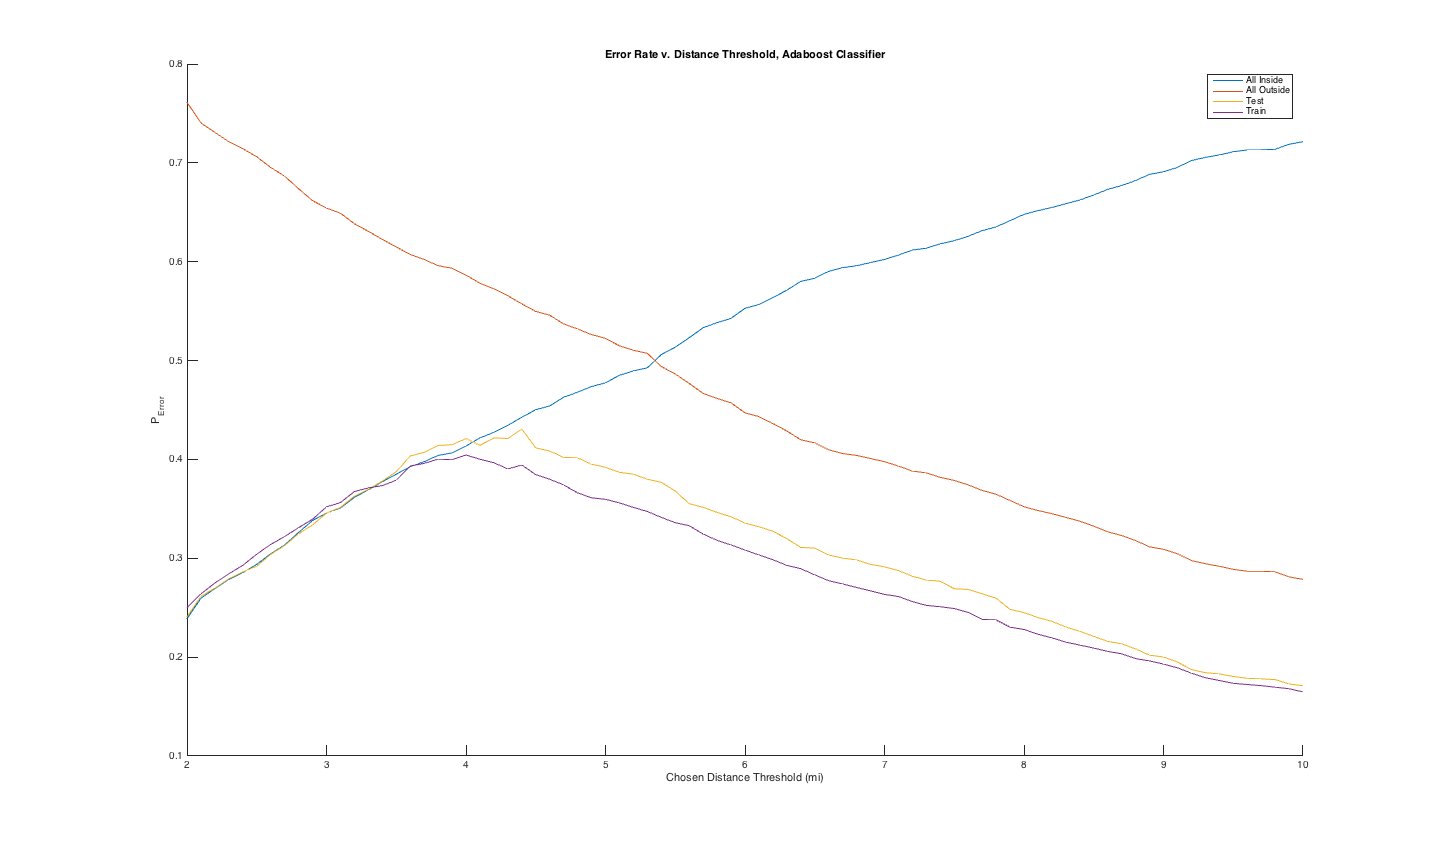
\includegraphics[width=0.9\linewidth]{adaboost_sweep_stumps_0_1_150iter_filtered}
  \caption{The Error vs. Threshold Plot for AdaBoost no longer follows the plotted asymptote as the threshold increases.}
\label{fig:Adaboost_Sweep}
\end{figure}

\subsection{Neural Network}

Additionally, we test our data set using a standard neural network trained via
stochastic gradient descent with backpropagation. Our ANN is designed to
optimize the cross entropy loss and utilizes a rectified linear unit activation
function with an experimentally chosen network size of two hidden layers with
unit counts 5 on layer 1 and 3 on layer 1. After processing the learning
algorithm with around 12,000 iterations, or two full runs through the training
data, the network was able to achieve a 32.6\% prediction error rate on the
training set and 34.1\% prediction error rate on the test set. This experiment
was repeated for a few partitions of cross validation which yielded similar
measurements.

\subsection{Regression}

Finally, we tried to implement a type of regression, instead of a classifier. Ideally, with this problem we could train a regressor that, when given a business, could determine the distance that the given business was relative to a college campus.

Similar regressors have been developed previously
\cite{Neural_Network_Regression}, and the tools from this class were helpful in
developing the backpropagation equations that were necessary for this system to
work. To visualize what the Neural Network was that we were training, we have
included Figure~\ref{fig:regression_nn}.

\begin{figure}
  \centering
  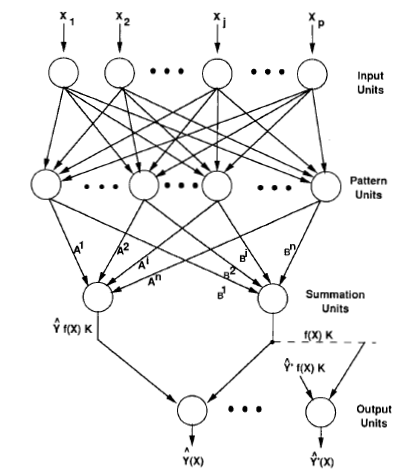
\includegraphics[width=0.9\linewidth]{regression_nn}
  \caption{A Neural Network Designed to Perform Regression}
\label{fig:regression_nn}
\end{figure}

Unfortunately, neither our custom built Neural Networks or those that were
created using packaged software could closely match the training labels when
trained on our training set.

In most cases, the neural network could somewhat closely match distances that
were greater than 1000 miles, however the range we were most interested in was
the 2 - 5 mile range. In the future, we would further tailor our data set to see
if the neural network would perform better with less outliers in the training
process.

\section{Conclusion}

\begin{table}[H]
  \centering
  \begin{tabular}{|c|c|c|}
    \hline
    Choice &         Training Error            & Test Error\tabularnewline
    \hline
    \hline
    \small{Estimate via Prior Distribution} &  49.1\%  & 49.0\% \tabularnewline
    \hline
    \small{Gaussian BDR Classifier}         &  26.4\%  & 35.7\% \tabularnewline
    \hline
    \small{AdaBoost with decision stumps}   &  35.2\%  & 38.4\% \tabularnewline
    \hline
    \small{Neural Network with ReLU}        &  32.6\%  & 34.1\%\tabularnewline
    \hline
  \end{tabular}
  \caption{Comparison of Classifiers.}\label{table:results_all_classifiers}
\end{table}

In all three of the attempted classification strategies, our algorithm was able
to achieve around 35\% error in the test data set. This is a significant
improvement compared to the trivial classifier based on prior probability
estimates alone (the split between the two classes was close to 50/50 for our
chosen distance threshold of 5.2 miles). Aside from minimizing error, each
classifier could be used to draw additional insights from the data.

Using the Gaussian classifier, we were able to identify a range of distance
thresholds that best separated the data into college-centric and
non-college-centric businesses. Continuing with Fisher's linear discriminant
analysis, we identified a tendency for restaurants near colleges to have
significantly more midday check-ins, particularly on Friday. We also several key
tags that were characteristic of college-oriented businesses, such as "Food
Trucks" and "Beer, Wine \& Spirits." Similar FLD analysis of the subtopics was
not as successful, producing some puzzling results that suggest further
adjustments that need to be made on our Latent Dirichlet Allocation algorithm.

In our AdaBoost tests, we found that the classifier performed relatively well
based on the check-in hours alone, which suggested that more pre-processing
could be applied to the restaurant tags and review subtopics to better condition
these features for classification, since the method we used resulted in a lot of
sparsity in the feature vectors for both restaurant tags and subtopics.

The neural network classifier was able to achieve the lowest error rate, but the
improvement over other methods was not significant. It is likely that our
dataset was simply too small (6000 training samples) to supply enough
information to the neural network. Applying our methods to general businesses
(not just restaurants) may yield better results, since the original unfiltered
Yelp dataset contained around 40,000 businesses.

Overall, the challenge of classifying restaurants near colleges was
best solved by Bayesian methods. Although the Gaussian BDR classifier may not
have performed as well as the neural network in terms of classification error,
we were able to draw many valuable insights by looking at the results with
Fisher's linear discriminant analysis. The ultimate goal of classifying these
restaurants was to identify trends in check-in hours, restaurant tags, and
subtopics mentioned in restaurant reviews, and by visualizing the discriminant
vector for each of these features, we were able to do exactly that.

\begin{thebibliography}{9}
  \bibitem{LDA_original}
    D. M. Blei, A. Y. Ng, M. I. Jordan, and J. Lafferty.
    Latent dirichlet allocation. \textit{Journal of Machine Learning Research},
    2003.
  \bibitem{LDA_Supervised}
    D. M. Blei and Jon D. McAuliffe. Supervised topic models.
    \textit{Advances in Neural Information Processing
    Systems}, 2007.
  \bibitem{Adaboost_original}
    Y. Freund and R. E. Schapire. A Decision-Theoretic Generalization of
    on-Line Learning and an Application to Boosting. \textit{J. Comput. Syst.
    Sci.}, 1993.
  \bibitem{cross_validation}
    R. Kohavi. A study of cross-validation and bootstrap for accuracy estimation
    and model selection. \textit{Ijcai}, 14(2), pp. 1137-1145. Aug 1995.
  \bibitem{FLD_kernels}
    B. Sch{\"o}lkopf and K. R. M{\"u}ller.
    Fisher Discriminant Analysis with Kernels. \textit{Neural networks for
    signal processing IX}, 1(1), Aug 1999.
  \bibitem{Neural_Network_Regression}
    D. F. Specht, "A general regression neural network," in \textit{IEEE
    Transactions on Neural Networks}, 2(6), pp. 568-576, Nov 1991.

\end{thebibliography}

\bibliographystyle{ieee}
\bibliography{egbib}

\end{document}
